\documentclass[letter,12pt]{article}
\usepackage[T1]{fontenc}
\usepackage[utf8]{inputenc}
\usepackage{lmodern}
\usepackage{hyperref}
\usepackage[english]{babel}
\usepackage{fourier}
\usepackage[protrusion=true,expansion=true]{microtype}
\usepackage{amsmath,amsfonts,amsthm}
\usepackage[pdftex]{graphicx}
\usepackage{sectsty}								
\usepackage[svgnames]{xcolor}			
%\allsectionsfont{\centering \normalfont\scshape}	
\usepackage{fancyhdr}
\usepackage{fancyvrb }


\makeatletter
\def\PY@reset{\let\PY@it=\relax \let\PY@bf=\relax%
    \let\PY@ul=\relax \let\PY@tc=\relax%
    \let\PY@bc=\relax \let\PY@ff=\relax}
\def\PY@tok#1{\csname PY@tok@#1\endcsname}
\def\PY@toks#1+{\ifx\relax#1\empty\else%
    \PY@tok{#1}\expandafter\PY@toks\fi}
\def\PY@do#1{\PY@bc{\PY@tc{\PY@ul{%
    \PY@it{\PY@bf{\PY@ff{#1}}}}}}}
\def\PY#1#2{\PY@reset\PY@toks#1+\relax+\PY@do{#2}}

\expandafter\def\csname PY@tok@gd\endcsname{\def\PY@tc##1{\textcolor[rgb]{0.63,0.00,0.00}{##1}}}
\expandafter\def\csname PY@tok@gu\endcsname{\let\PY@bf=\textbf\def\PY@tc##1{\textcolor[rgb]{0.50,0.00,0.50}{##1}}}
\expandafter\def\csname PY@tok@gt\endcsname{\def\PY@tc##1{\textcolor[rgb]{0.00,0.27,0.87}{##1}}}
\expandafter\def\csname PY@tok@gs\endcsname{\let\PY@bf=\textbf}
\expandafter\def\csname PY@tok@gr\endcsname{\def\PY@tc##1{\textcolor[rgb]{1.00,0.00,0.00}{##1}}}
\expandafter\def\csname PY@tok@cm\endcsname{\let\PY@it=\textit\def\PY@tc##1{\textcolor[rgb]{0.25,0.50,0.50}{##1}}}
\expandafter\def\csname PY@tok@vg\endcsname{\def\PY@tc##1{\textcolor[rgb]{0.10,0.09,0.49}{##1}}}
\expandafter\def\csname PY@tok@m\endcsname{\def\PY@tc##1{\textcolor[rgb]{0.40,0.40,0.40}{##1}}}
\expandafter\def\csname PY@tok@mh\endcsname{\def\PY@tc##1{\textcolor[rgb]{0.40,0.40,0.40}{##1}}}
\expandafter\def\csname PY@tok@go\endcsname{\def\PY@tc##1{\textcolor[rgb]{0.53,0.53,0.53}{##1}}}
\expandafter\def\csname PY@tok@ge\endcsname{\let\PY@it=\textit}
\expandafter\def\csname PY@tok@vc\endcsname{\def\PY@tc##1{\textcolor[rgb]{0.10,0.09,0.49}{##1}}}
\expandafter\def\csname PY@tok@il\endcsname{\def\PY@tc##1{\textcolor[rgb]{0.40,0.40,0.40}{##1}}}
\expandafter\def\csname PY@tok@cs\endcsname{\let\PY@it=\textit\def\PY@tc##1{\textcolor[rgb]{0.25,0.50,0.50}{##1}}}
\expandafter\def\csname PY@tok@cp\endcsname{\def\PY@tc##1{\textcolor[rgb]{0.74,0.48,0.00}{##1}}}
\expandafter\def\csname PY@tok@gi\endcsname{\def\PY@tc##1{\textcolor[rgb]{0.00,0.63,0.00}{##1}}}
\expandafter\def\csname PY@tok@gh\endcsname{\let\PY@bf=\textbf\def\PY@tc##1{\textcolor[rgb]{0.00,0.00,0.50}{##1}}}
\expandafter\def\csname PY@tok@ni\endcsname{\let\PY@bf=\textbf\def\PY@tc##1{\textcolor[rgb]{0.60,0.60,0.60}{##1}}}
\expandafter\def\csname PY@tok@nl\endcsname{\def\PY@tc##1{\textcolor[rgb]{0.63,0.63,0.00}{##1}}}
\expandafter\def\csname PY@tok@nn\endcsname{\let\PY@bf=\textbf\def\PY@tc##1{\textcolor[rgb]{0.00,0.00,1.00}{##1}}}
\expandafter\def\csname PY@tok@no\endcsname{\def\PY@tc##1{\textcolor[rgb]{0.53,0.00,0.00}{##1}}}
\expandafter\def\csname PY@tok@na\endcsname{\def\PY@tc##1{\textcolor[rgb]{0.49,0.56,0.16}{##1}}}
\expandafter\def\csname PY@tok@nb\endcsname{\def\PY@tc##1{\textcolor[rgb]{0.00,0.50,0.00}{##1}}}
\expandafter\def\csname PY@tok@nc\endcsname{\let\PY@bf=\textbf\def\PY@tc##1{\textcolor[rgb]{0.00,0.00,1.00}{##1}}}
\expandafter\def\csname PY@tok@nd\endcsname{\def\PY@tc##1{\textcolor[rgb]{0.67,0.13,1.00}{##1}}}
\expandafter\def\csname PY@tok@ne\endcsname{\let\PY@bf=\textbf\def\PY@tc##1{\textcolor[rgb]{0.82,0.25,0.23}{##1}}}
\expandafter\def\csname PY@tok@nf\endcsname{\def\PY@tc##1{\textcolor[rgb]{0.00,0.00,1.00}{##1}}}
\expandafter\def\csname PY@tok@si\endcsname{\let\PY@bf=\textbf\def\PY@tc##1{\textcolor[rgb]{0.73,0.40,0.53}{##1}}}
\expandafter\def\csname PY@tok@s2\endcsname{\def\PY@tc##1{\textcolor[rgb]{0.73,0.13,0.13}{##1}}}
\expandafter\def\csname PY@tok@vi\endcsname{\def\PY@tc##1{\textcolor[rgb]{0.10,0.09,0.49}{##1}}}
\expandafter\def\csname PY@tok@nt\endcsname{\let\PY@bf=\textbf\def\PY@tc##1{\textcolor[rgb]{0.00,0.50,0.00}{##1}}}
\expandafter\def\csname PY@tok@nv\endcsname{\def\PY@tc##1{\textcolor[rgb]{0.10,0.09,0.49}{##1}}}
\expandafter\def\csname PY@tok@s1\endcsname{\def\PY@tc##1{\textcolor[rgb]{0.73,0.13,0.13}{##1}}}
\expandafter\def\csname PY@tok@kd\endcsname{\let\PY@bf=\textbf\def\PY@tc##1{\textcolor[rgb]{0.00,0.50,0.00}{##1}}}
\expandafter\def\csname PY@tok@sh\endcsname{\def\PY@tc##1{\textcolor[rgb]{0.73,0.13,0.13}{##1}}}
\expandafter\def\csname PY@tok@sc\endcsname{\def\PY@tc##1{\textcolor[rgb]{0.73,0.13,0.13}{##1}}}
\expandafter\def\csname PY@tok@sx\endcsname{\def\PY@tc##1{\textcolor[rgb]{0.00,0.50,0.00}{##1}}}
\expandafter\def\csname PY@tok@bp\endcsname{\def\PY@tc##1{\textcolor[rgb]{0.00,0.50,0.00}{##1}}}
\expandafter\def\csname PY@tok@c1\endcsname{\let\PY@it=\textit\def\PY@tc##1{\textcolor[rgb]{0.25,0.50,0.50}{##1}}}
\expandafter\def\csname PY@tok@kc\endcsname{\let\PY@bf=\textbf\def\PY@tc##1{\textcolor[rgb]{0.00,0.50,0.00}{##1}}}
\expandafter\def\csname PY@tok@c\endcsname{\let\PY@it=\textit\def\PY@tc##1{\textcolor[rgb]{0.25,0.50,0.50}{##1}}}
\expandafter\def\csname PY@tok@mf\endcsname{\def\PY@tc##1{\textcolor[rgb]{0.40,0.40,0.40}{##1}}}
\expandafter\def\csname PY@tok@err\endcsname{\def\PY@bc##1{\setlength{\fboxsep}{0pt}\fcolorbox[rgb]{1.00,0.00,0.00}{1,1,1}{\strut ##1}}}
\expandafter\def\csname PY@tok@mb\endcsname{\def\PY@tc##1{\textcolor[rgb]{0.40,0.40,0.40}{##1}}}
\expandafter\def\csname PY@tok@ss\endcsname{\def\PY@tc##1{\textcolor[rgb]{0.10,0.09,0.49}{##1}}}
\expandafter\def\csname PY@tok@sr\endcsname{\def\PY@tc##1{\textcolor[rgb]{0.73,0.40,0.53}{##1}}}
\expandafter\def\csname PY@tok@mo\endcsname{\def\PY@tc##1{\textcolor[rgb]{0.40,0.40,0.40}{##1}}}
\expandafter\def\csname PY@tok@kn\endcsname{\let\PY@bf=\textbf\def\PY@tc##1{\textcolor[rgb]{0.00,0.50,0.00}{##1}}}
\expandafter\def\csname PY@tok@mi\endcsname{\def\PY@tc##1{\textcolor[rgb]{0.40,0.40,0.40}{##1}}}
\expandafter\def\csname PY@tok@gp\endcsname{\let\PY@bf=\textbf\def\PY@tc##1{\textcolor[rgb]{0.00,0.00,0.50}{##1}}}
\expandafter\def\csname PY@tok@o\endcsname{\def\PY@tc##1{\textcolor[rgb]{0.40,0.40,0.40}{##1}}}
\expandafter\def\csname PY@tok@kr\endcsname{\let\PY@bf=\textbf\def\PY@tc##1{\textcolor[rgb]{0.00,0.50,0.00}{##1}}}
\expandafter\def\csname PY@tok@s\endcsname{\def\PY@tc##1{\textcolor[rgb]{0.73,0.13,0.13}{##1}}}
\expandafter\def\csname PY@tok@kp\endcsname{\def\PY@tc##1{\textcolor[rgb]{0.00,0.50,0.00}{##1}}}
\expandafter\def\csname PY@tok@w\endcsname{\def\PY@tc##1{\textcolor[rgb]{0.73,0.73,0.73}{##1}}}
\expandafter\def\csname PY@tok@kt\endcsname{\def\PY@tc##1{\textcolor[rgb]{0.69,0.00,0.25}{##1}}}
\expandafter\def\csname PY@tok@ow\endcsname{\let\PY@bf=\textbf\def\PY@tc##1{\textcolor[rgb]{0.67,0.13,1.00}{##1}}}
\expandafter\def\csname PY@tok@sb\endcsname{\def\PY@tc##1{\textcolor[rgb]{0.73,0.13,0.13}{##1}}}
\expandafter\def\csname PY@tok@k\endcsname{\let\PY@bf=\textbf\def\PY@tc##1{\textcolor[rgb]{0.00,0.50,0.00}{##1}}}
\expandafter\def\csname PY@tok@se\endcsname{\let\PY@bf=\textbf\def\PY@tc##1{\textcolor[rgb]{0.73,0.40,0.13}{##1}}}
\expandafter\def\csname PY@tok@sd\endcsname{\let\PY@it=\textit\def\PY@tc##1{\textcolor[rgb]{0.73,0.13,0.13}{##1}}}

\def\PYZbs{\char`\\}
\def\PYZus{\char`\_}
\def\PYZob{\char`\{}
\def\PYZcb{\char`\}}
\def\PYZca{\char`\^}
\def\PYZam{\char`\&}
\def\PYZlt{\char`\<}
\def\PYZgt{\char`\>}
\def\PYZsh{\char`\#}
\def\PYZpc{\char`\%}
\def\PYZdl{\char`\$}
\def\PYZhy{\char`\-}
\def\PYZsq{\char`\'}
\def\PYZdq{\char`\"}
\def\PYZti{\char`\~}
% for compatibility with earlier versions
\def\PYZat{@}
\def\PYZlb{[}
\def\PYZrb{]}
\makeatother



\pagestyle{fancyplain}
\fancyhead{}	
\fancyfoot[L]{\small \url{http://toddvance.tech}}		
\fancyfoot[C]{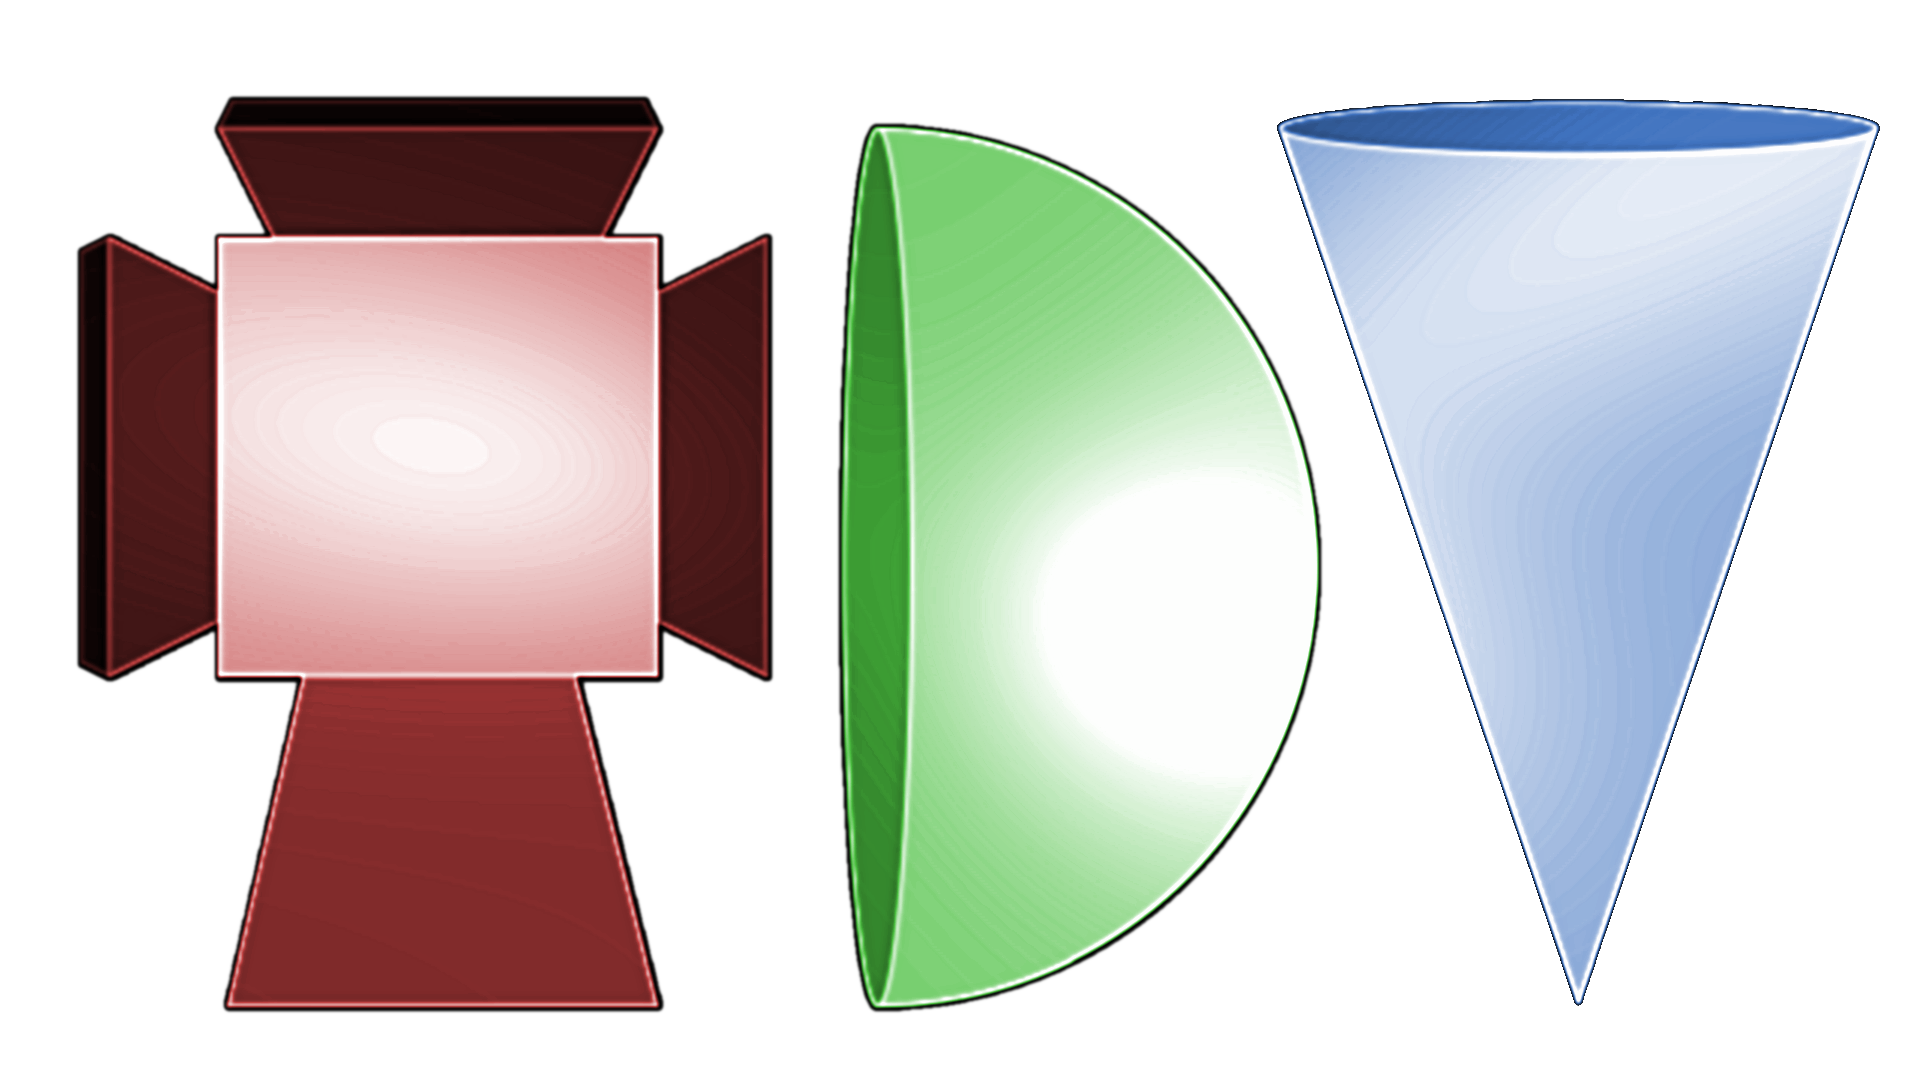
\includegraphics[width=0.5in]{monogram-transparent.png}}											
\fancyfoot[R]{\thepage}								
\renewcommand{\headrulewidth}{0pt}			
\renewcommand{\footrulewidth}{0pt}
\setlength{\headheight}{13.6pt}
\newcommand{\horrule}[1]{\rule{\linewidth}{#1}} 	% Horizontal rule

\title{
		%\vspace{-1in}
		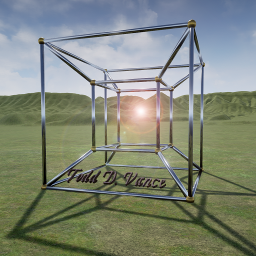
\includegraphics[width=1.5in]{tdv-logo-south-branch-valley-small.png}
		\usefont{OT1}{bch}{b}{n} 
		\normalfont 
		\horrule{0.5pt} \\[0.4cm]
		\Huge Game State Machine\\ %%%%%%%%%%%%%% TITLE %%%%%%%%%%%%%%%
		\color{DarkGreen}
		\large User’s Manual\\[0.2cm]%%%%%%%%%%%%%%ARTICLE TYPE %%%%%%%%%%%%%%%
		\color{Blue}
		\small \textsc{Add state to video games}\\%%%%%%%%%%%%%% TAG LINE %%%%%%%%%%%%%%%
		\color{Black}
		\horrule{2pt} \\[0.5cm]
}
\author{
		\normalfont \normalsize
       \copyright{2017 Todd D. Vance}%%%%%%%%%%%%%% COPYRIGHT %%%%%%%%%%%%%%%
        \tiny\\
\tiny        Permission is hereby granted, free of charge, to any person obtaining a copy\\[-0.3cm]
\tiny        of this software and associated documentation files (the "Software"), to deal\\[-0.3cm] 
\tiny        in the Software without restriction, including without limitation the rights to\\[-0.3cm]
\tiny         use, copy, modify, merge, publish, distribute, sublicense, and/or sell copies\\[-0.3cm] 
\tiny         of the Software, and to permit persons to whom the Software is furnished to\\[-0.3cm]
\tiny         do so, subject to the following conditions:\\[-0.3cm]
\tiny         \\[-0.3cm]
\tiny	The above copyright notice and this permission notice shall be included in all\\[-0.3cm]
\tiny	copies or substantial portions of the Software.\\[-0.3cm]
\tiny	\\[-0.3cm]
\tiny	THE SOFTWARE IS PROVIDED "AS IS", WITHOUT WARRANTY OF ANY KIND,\\[-0.3cm]
\tiny	EXPRESS OR IMPLIED, INCLUDING BUT NOT LIMITED TO THE WARRANTIES\\[-0.3cm] 
\tiny	OF MERCHANTABILITY, FITNESS FOR A PARTICULAR PURPOSE AND\\[-0.3cm]
\tiny	NONINFRINGEMENT. IN NO EVENT SHALL THE AUTHORS OR COPYRIGHT\\[-0.3cm]
\tiny	HOLDERS BE LIABLE FOR ANY CLAIM, DAMAGES OR OTHER LIABILITY,\\[-0.3cm]
\tiny	WHETHER IN AN ACTION OF CONTRACT, TORT OR OTHERWISE, ARISING\\[-0.3cm]
\tiny	FROM, OUT OF OR IN CONNECTION WITH THE SOFTWARE OR THE USE\\[-0.3cm]
\tiny   OR OTHER DEALINGS IN THE SOFTWARE.
}
\date{January 1, 2017}

\begin{document}
\maketitle{}
\tableofcontents{}

%%%%%%%%%%%%%% BEGIN DOCUMENT %%%%%%%%%%%%%%%

\section{What is a State Machine}

A Finite State Machine, more technically called a Deterministic Finite Automaton is a theoretical concept that models a simple robot that follows simple rules: it is in a state; it receives an input; Based on the current state and the input, it does something, and it goes into a new state (or the same state again).  It has been “invented” many times in many different forms over the centuries (Euclid’s straightedge and compass constructions are probably the earliest), but the most common model used in computer programming, similar to the one used here (we actually use a variant, called the Mealy model), was first described in detail in the mid 20th century scholarly paper: Moore, Edward F (1956). "Gedanken-experiments on Sequential Machines". Automata Studies, Annals of Math. Studies. Princeton, N.J.: Princeton University Press (34): 129–153.  (A “Gedanken-experiment” is a thought experiment, done in the head instead of in a laboratory).
In real life, finite state machines occur in lots of everyday products, nowadays controlled by computers but in earlier times, controlled by a mechanical process.  Examples include vending machines, automatic teller machines, stoplights, subway turnstyles, and simpler mechanical devices like mouse traps.

\subsection{Mouse Trap Model}


A very simple, mechanical example of a state machine is the standard mousetrap (not the modern techy humane ones—I don’t know how they work): it has two states, set (as shown in the image), and unset.  The inputs are mouse or no mouse, or “set the trap”.  The behaviors are spring, or do nothing.  If it is in the “unset” state, it does nothing, whether or not there is a mouse, and stays in the unset state.  If it is in the “set” state, it springs if a mouse is present and goes to the unset state.  If there is no mouse, it does nothing and remains in the set state.  If it is unset and a human does “set the trap”, it goes to the set state.  If it is set and the human does “set the trap”, this is really an error condition, and what actually happens might be that the trap springs and it goes to the unset state and the human learns his lesson.

\subsection{Game State Machine}
The particular state machine implemented by this asset is the overall game state machine.  This doesn’t have much to do with the details of game play, but of the organization of levels, cutscenes, title screens, and so on in a game.  Consider the classic arcade game Pac-Man for an example, whose game state machine is typical of many classic arcade games.

When you walked up to the game, it was most likely in “attract” mode, the mode that tries to get you to spend a quarter.  This is a big state that will be divided into smaller states (title, demo, and so on—note Namco/Bally probably have their own names for the states; I’m making up names that are reasonably descriptive).  But before the attract mode, there is another mode not seen often unless you pull the plug and plug it back in: booting up.

\begin{enumerate}

\item[Boot] This is the initial state, the start state of the game.  It takes a certain amount of time to finish, and when it does, it immediately transitions to the Title state.  Input is not noticed (although, for all I know, there might be special codes to do certain tests, etc. that the arcade operator could do at this point).

\item[Title] The screen that shows the title of the game and some graphics to make someone come closer for a better look.  After a certain amount of time has passed, it goes to the Description state.  If a quarter is spent and the Play button is pressed, it instead goes to the Start Game state.

\item[Description] Here is a screen describing game play and points for various activities.  After a certain amount of time has passed, it goes to the High Scores state (I might have Description and High Scores in the wrong order; it has been decades since I’ve played Pac-Man at an arcade).  If a quarter is spent and the Play button is pressed, it instead goes to the Start Game state.

\item[High Scores] The top ten scores, with initials, are displayed here.  After a certain amount of time has passed, it goes to the Demo state.  If a quarter is spent and the Play button is pressed, it instead goes to the Start Game state.

\item[Demo] A sample game is shown, without sounds and possibility for player input.  It doesn’t last long before Pac-Man is eaten and the game returns to the Title state.  If a quarter is spent and the Play button is pressed, it instead goes to the Start Game state.

\item[Start Game] The Level 1 board is displayed, the intro music is played, Pac Man and the ghosts appear on the board, and then the game transitions to the Play Game state.  Input is ignored during the Start Game state.

\item[Play Game] Now the input is connected to the game and a user can play.  Depending on the events of the game, the next state is Level Up or Game Over (recall, this is just overall game state, we are not modeling the fine points of game play at his level).

\item[Level Up] When the board is cleared, this state is entered.  The board flashes, and there may be a cutscene.  When this is done, the next level is loaded and the game goes back to Play Game.

\item[Game Over] When the player runs out of lives, the game is over.  A big Game Over message appears over top the game board while the ghosts dance in glee at having earned another quarter.  After a time, one of two things happen.  Either it returns directly to the Title state, or if the score achieved is in the top ten, it goes to the New High Score state.

\item[New High Score] The player is given the opportunity to enter his initials to appear on the high score board.  After the initials are entered (or if it times out with it stuck on AAA, since some players just walk away), the game returns to the High Score state--or rather, a duplicate of the High Score state (I’ll call it High Scores Reprise) that transitions to the Title rather than to the Demo.

\item[High Scores Reprise] The top ten scores, with initials, are displayed here, with the just-made high score highlighted.  After a certain amount of time has passed, it goes to the Title state.  If a quarter is spent and the Play button is pressed, it instead goes to the Start Game state.
\end{enumerate}

\section{Features}

\begin{itemize}
\item Singleton class loaded once and persistent through scene changes
\item Parses a state machine specification from a plain text file
\item Easy to read, easy to write mini-language to specify a state machine; syntax is like C function calls
\item Transition to a new state after a certain time has elapsed
\item Transition to a new state after a certain event is received
\item Go back in the history of states visited
\item Optionally load a scene upon entering a state (additive loading supported)
\item Optionally log what the state machine is doing

\end{itemize}


\section{Walk-Through: Setting Up a State Machine for a Game}

This walk-through is done using Unity 5.5.0f3 on Windows 10.  Other situations should be comparable.

\subsection{Create a new, empty project}

\begin{figure}
 \includegraphics[width=6in]{layout.png}
 \caption{Unity3D With The Default Layout}
 \label{fig:layout}
\end{figure}


\begin{enumerate}

\item First, open the Unity3d program.  After a short period of time, a “Projects” menu should show (this may look different if you have not saved any previous projects for Unity3d).

\item Click the New button (the icon is a dog-eared sheet of paper with a plus sign in it).

\item Three fields will call for input: Project name, Location, and Organization.  The last will be filled in if you have registered the software.  Choose any name and organization for the project.  For example, one might call it “GSM\_Walkthrough”.  

\item It doesn’t matter at this point whether it is 3D or 2D, or if Unity Analytics are enabled.  There is no need to add any asset packages yet.

\item Click the bluish-green “Create Project” button to get started.  After a moment of setup, Unity will open its IDE using some starting layout. 

\item To ensure the reader and the author are on the same page, click the Layout button at the top, all the way to the right, and ensure it is set to “Default”.  The screen at this point will look like Figure \ref{fig:layout} 

\end{enumerate}

\subsection{Import the Asset}

\begin{figure}
 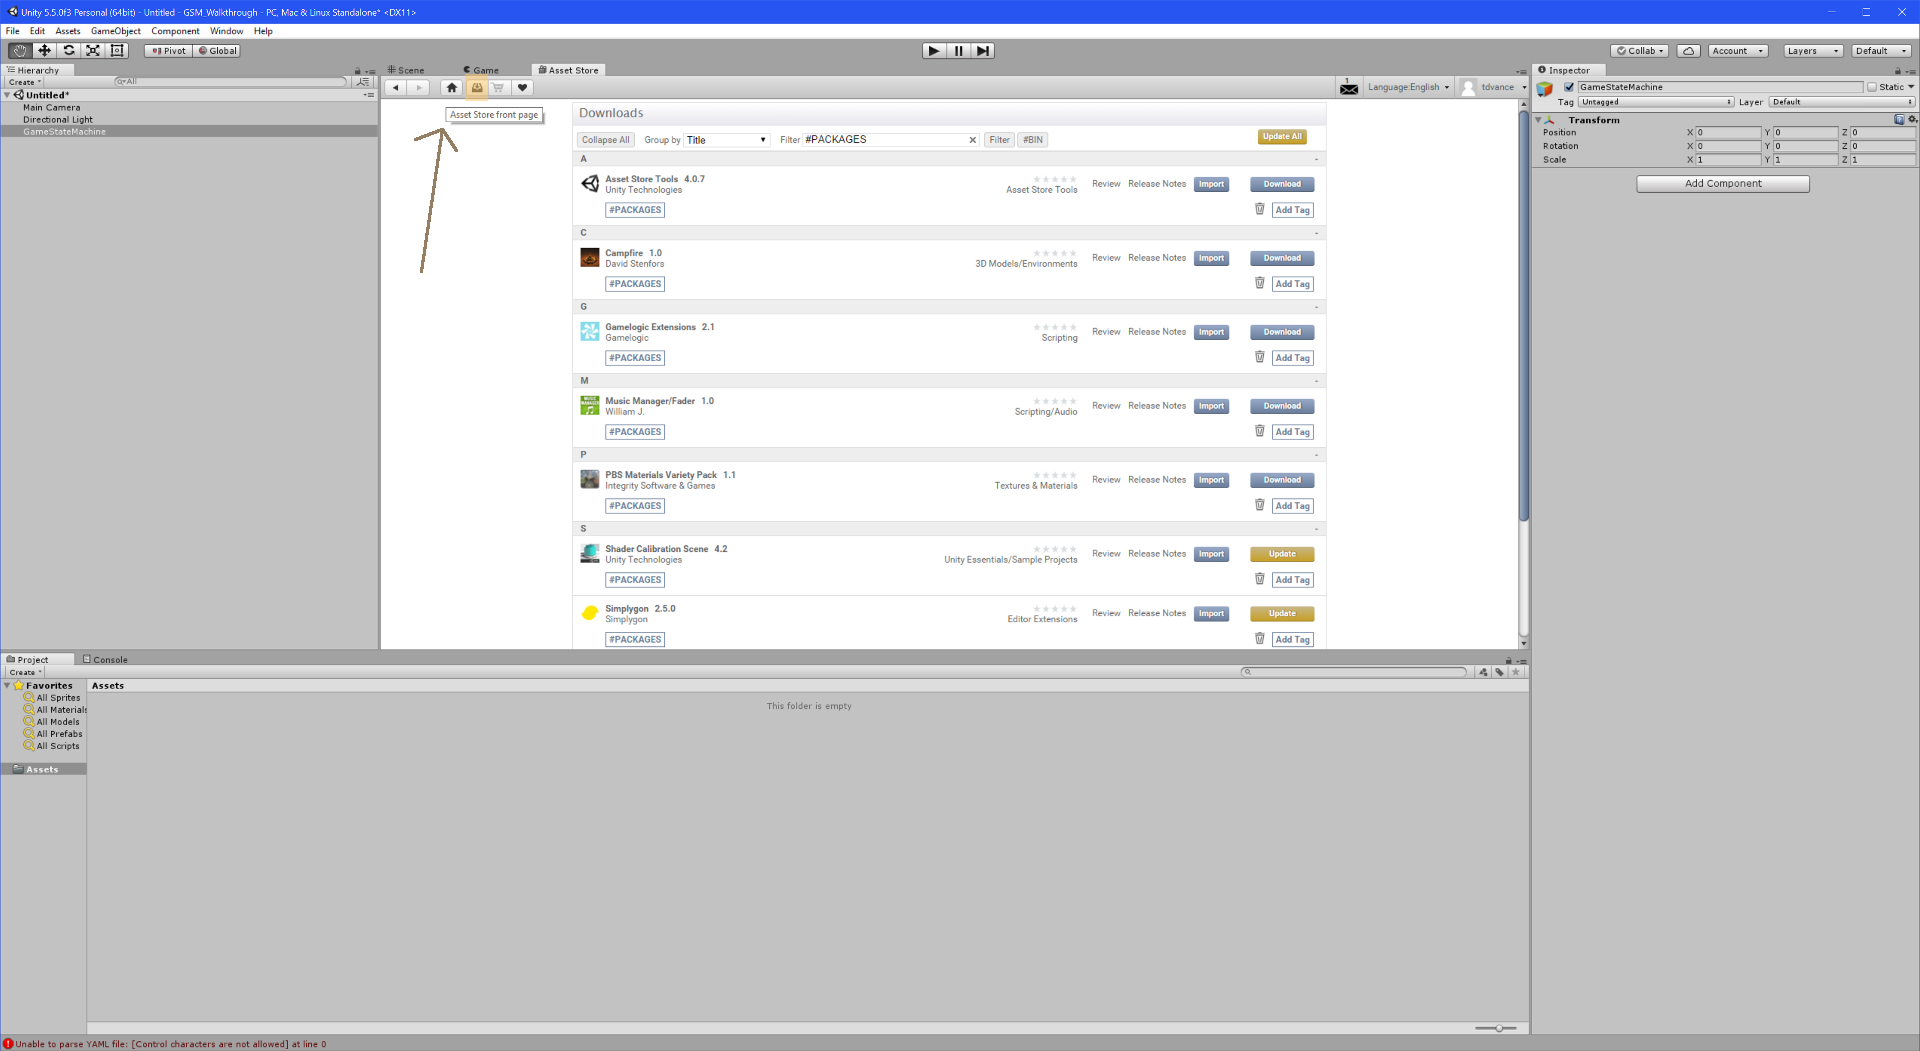
\includegraphics[width=6in]{asset.png}
 \caption{Asset Store Download Manager}
 \label{fig:asset}
\end{figure}

\begin{enumerate}

\item This assumes you already have the GameStateMachine asset purchased (it’s free) from the Asset Store.  Click the Asset Store tab above the Scene window to show the Asset Store.  See Figure \ref{fig:asset}

\item At the top is an icon bar with severl icons.  If you hover over the icon that looks like a box with a downward-pointing arrow in it, it will show the tooltip “ToggleDownloadManager”.  Click this to bring up the Download Manager.  

\item Scroll down and find the GameStateMachine asset.  There are several buttons: “Import” and either “Update” or “Download”.  If the “Import” button is grayed out, you probably have to click “Download” first.  If the “Update” button shows, you might want to go ahead and update the asset before importing it.  Most of the time you need to do neither.

\item Click the Import button on the GameStateMachine asset to import it into your project.

\item Click the Scene tab at the top to bring back the Scene window.
 
\end{enumerate}

\subsection{Set up a starting scene}

\begin{figure}
 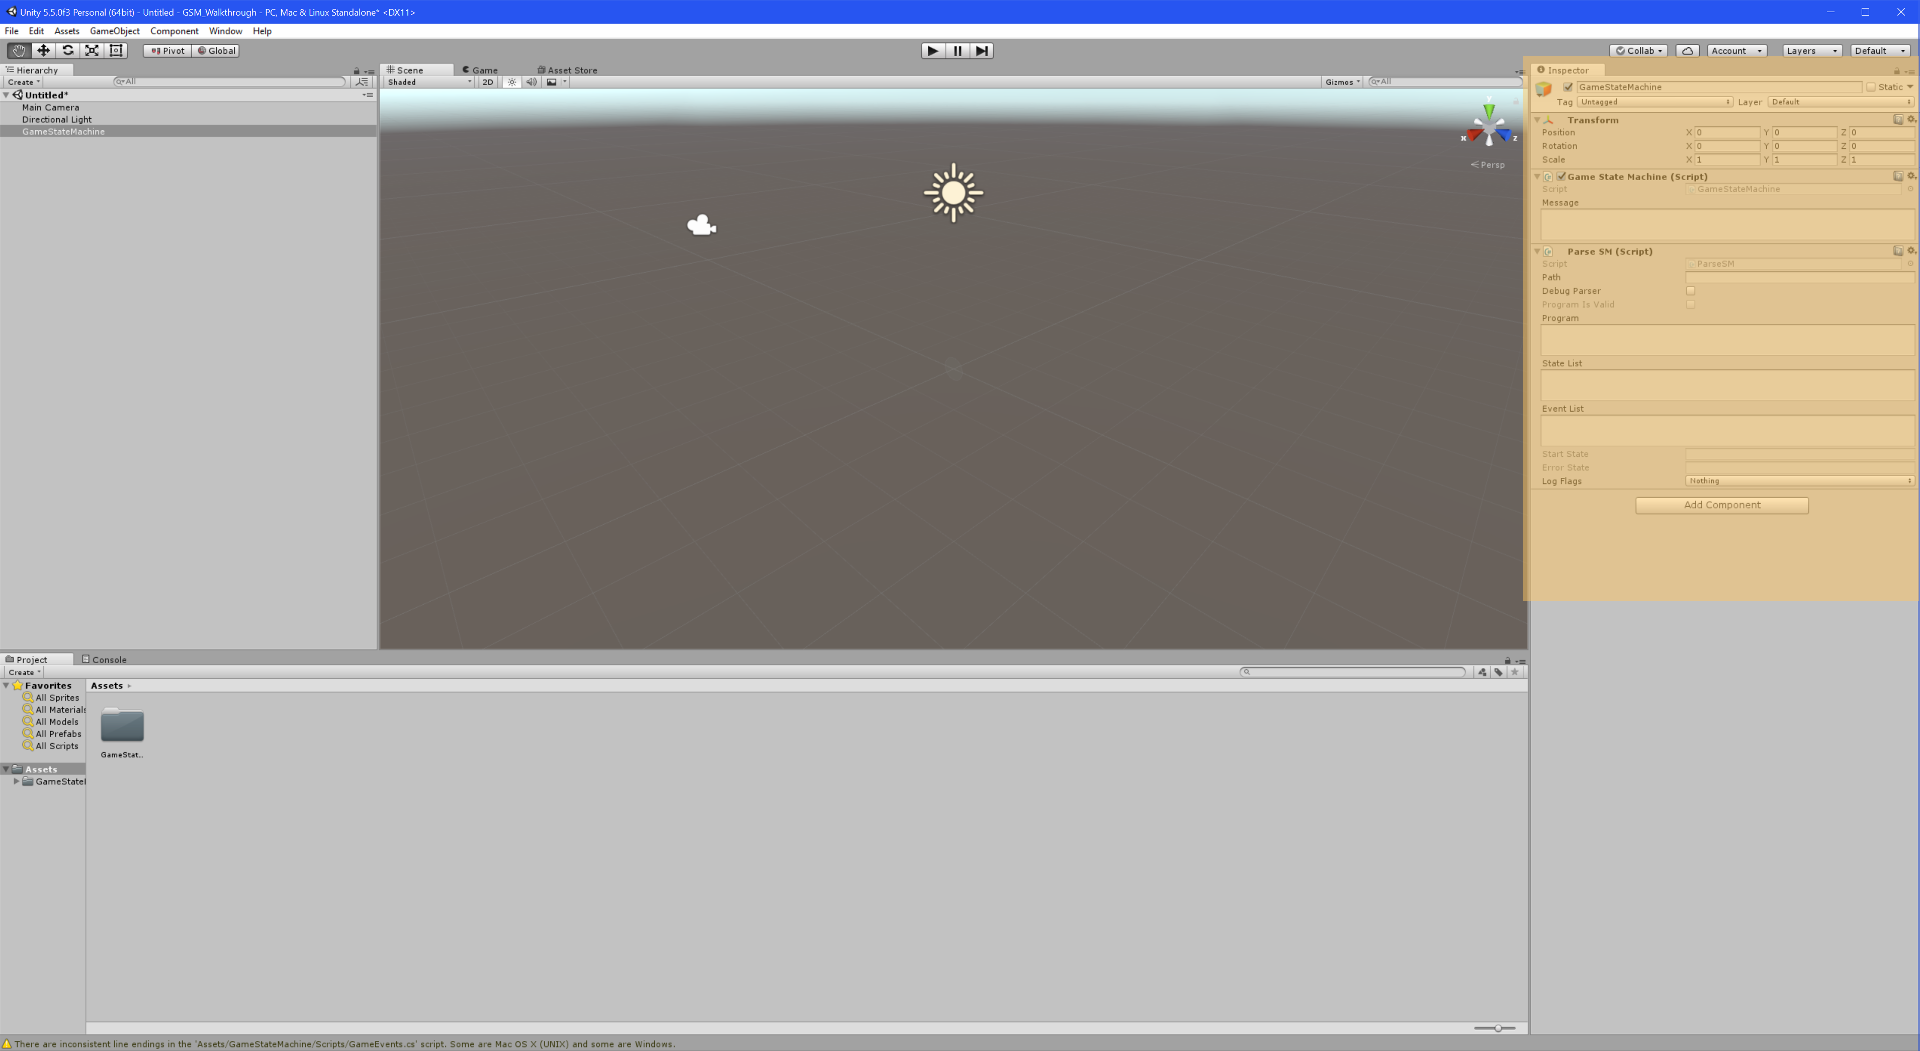
\includegraphics[width=6in]{inspector.png}
 \caption{GameStateMachine object with its components}
 \label{fig:inspector}
\end{figure}

The GameStateMachine class is a singleton so it should be loaded once in an initial scene that is never returned to again.  The steps are, in summary, create an empty game object, and add the “ParseSM” and “GameStateMachine” scripts to it as components.

\begin{enumerate}
\item Just under the Hierarchy tab on the left side, there is a “Create” button.  Click that, and select “Create Emtpy”.

\item A new item called “GameObject” should appear in the Hierarchy and should already be selected.  So, hit the F2 key and change its name to “GameStateMachine”.

\item While “GameStateMachine” is still selected, in the “Selector” on the right are the components of the “GameStateMachine” object.  Currently it has one component, the “Transform”.   Click the “Add Component” button and type in “GameStateMachine” and select the Game State Machine behaviour script (with a “C\#” icon to its left).  

\item “GameStateMachine” is still selected, again click the  “Add Component” button and type in “ParseSM” and select the “Parse SM” behaviour script (with a “C\#” icon to its left).  Now “GameStateMachine” has three components: “Transform”, “Game State Machine”, and “Parse SM”.  See Figure \ref{fig:inspector}

\item Click “Ctrl-S” to save the scene.  Choose a name like “Init”.

\item If you click the “Run” right-arrow button at the top center, nothing much will happen, because no state machine has been selected.  If “GameStateMachine” is still highlighted in the Hierarchy, it will show as “checked” the property “Program Is Valid”, because an empty program, while useless, is valid.  The other boxes will show information about the state machine being used, once we give it one.

\end{enumerate}

\subsection{Creating a State Machine}

\begin{figure}
 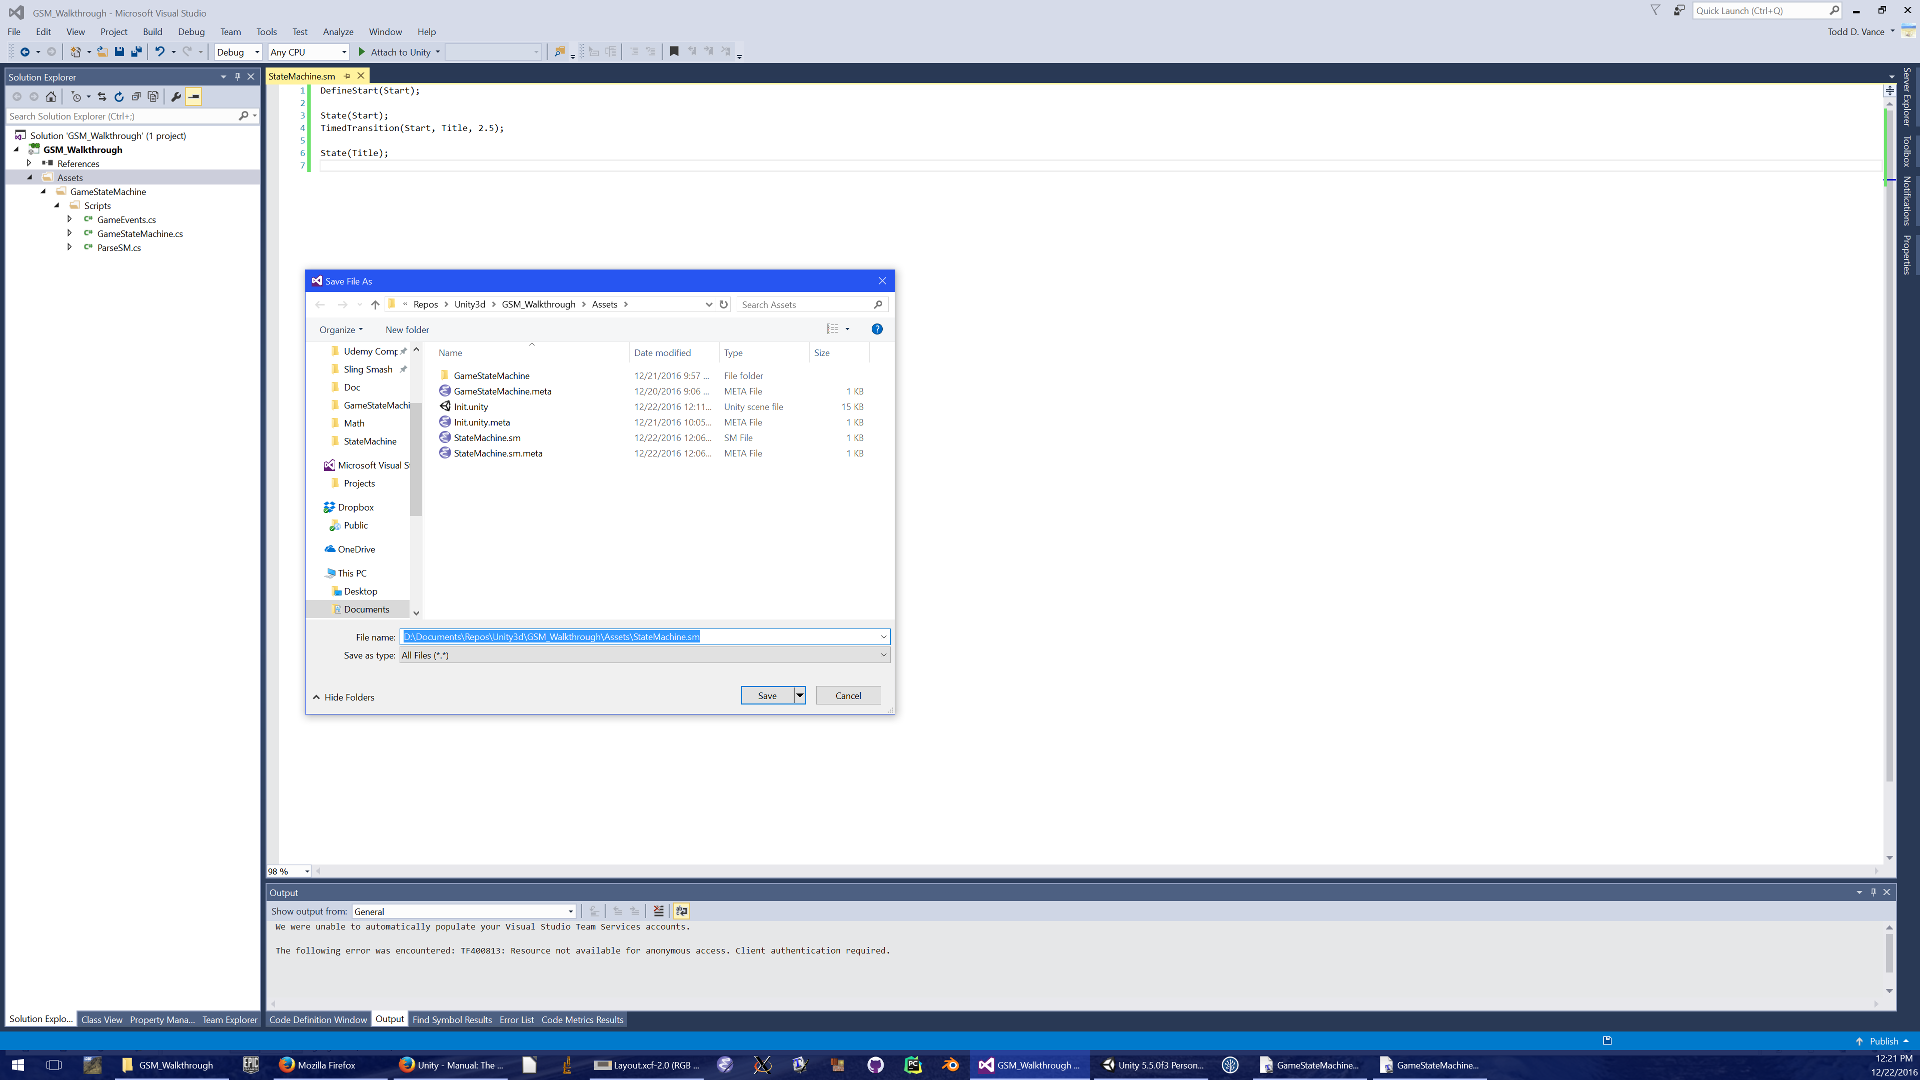
\includegraphics[width=6in]{vs.png}
 \caption{Program for the State Machine}
 \label{fig:vs}
\end{figure}

To create the state machine, we need to create a new file for the program.  To do so, you need a text editor.  Because most PC users of Unity use Visual Studio 2015, that is what is used in this walk-through.  MonoDevelop probably has similar 
capabilities.

\begin{enumerate}
\item Open the Visual Studio 2015 solution for this product.  The easiest way to do this is to follow the following steps.
	\begin{enumerate}
	\item In the Project window, ensure you are at the top directory level  “Assets”.
	\item In the Project window, right-click and select “Show in Explorer”.
	\item Explorer should open showing your project directory (“GSM\_Walkthrough” if you followed the author’s naming).  If not, you may have to navigate up a folder or so using the up-arrow icon to the left of the folder location breadcrumbs near the top just below the ribbon.
	\item Doubleclick the solution file ending in “.sln” (if following the author’s naming conventions, this would be the “GSM\_Walkthrough.sln” file--if you have “hide extensions” enabled, you might not see the “.sln” extension; but the icon to the left of the proper file has the “Visual Studio” symbol that looks like a purple $\infty$ sign made with triangles.)  If all is well, Visual Studio will open.
	\end{enumerate}
\item In Visual Studio, click File $\rightarrow$ New $\rightarrow$ File... $\rightarrow$ Text File.  This will open a new, blank text file.
\item Click File $\rightarrow$ Save <name of file> as....  Click the “Assets” folder so we save the state machine file into the Assets folder where it will show up in the Project window of Unity.  Then in the dropdown at the bottom, change the selection from Text File (.txt) to All Files (*.*).  Then, type a name for the file, such as “StateMachine.sm” (the convention is state machine files end in the “.sm” extension) and click the “Save” button to save the file under the new name.
\item Let us make a simple state machine with a four-line program.  Enter the following lines into the StateMachine.sm editor window in Visual Studio:

\begin{verbatim}
DefineStart(Start);

State(Start);
TimedTransition(Start, Title, 2.5);

State(Title);
\end{verbatim}

This state machine has two states, declared by the “State()” commands.   The “DefineStart" command makes the state called “Start” the initial state the machine is in when it is loaded.  After 2.5 seconds, the “Start” state will transition to the “Title” state.  Other than that, it does nothing.  See Figure \ref{fig:vs} for a screenshot of this stage.

\item After checking for typos and mistakes, click “Ctrl-S” to save the file.

\end{enumerate}

\subsection{Wire up the State Machine program to the State Machine}

\begin{figure}
 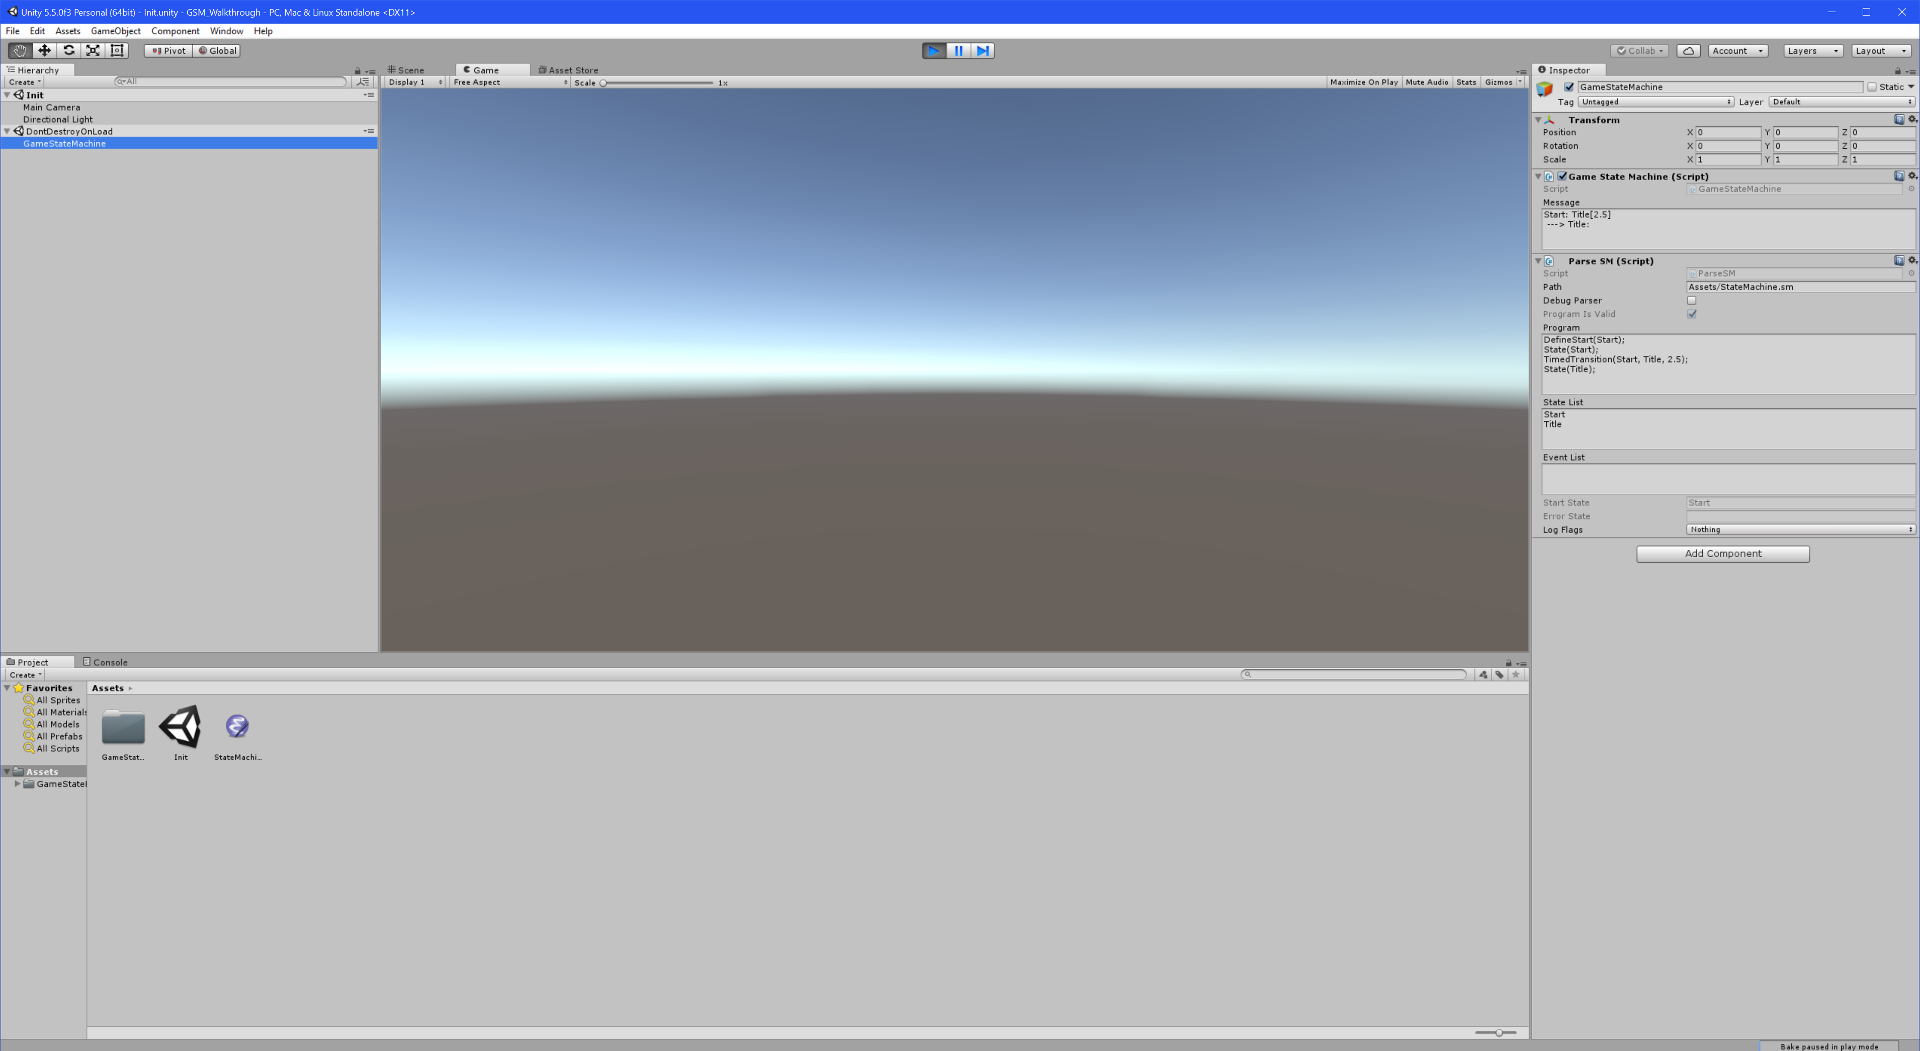
\includegraphics[width=6in]{final.png}
 \caption{GameStateMachine In Action}
 \label{fig:vs}
\end{figure}
\begin{enumerate}
\item Go back to the Unity3D editor.  If you followed the directions up to this point, there should be a StateMachine file in the Projects window, which should still be at the top Assets level.

\item Click the GameStateMachine game object in the Hierarchy window to bring it up in the inspector.

\item In the inspector, under the “Parse SM” component, is a text field called “path”.  Type in the path (relative to the project directory) of the state machine file.  If you followed the directions to this point, that path will be: “Assets/StateMachine.sm”.

\item Now, at the top center of the Unity window is the Run/Pause/Step icon group.  Click the Run icon (which looks like a triangle pointing to the right).  If everything is correct, the “Program Is Valid” property checkbox will be checked, indicating that there are no compile errors in the state machine.  In addition, the commands of the state machine program will show up in the Program textbox.  This is the program as the state machine parser sees it, minus white space and comments, and with capitalization “normalized”.  This can be used to check that the state machine the parser sees is what you think it is.  The “States” window shows the two states defined for this state machine.  Finally, in the Game State Machine component, you saee a different representation of the state machine, with an arrow pointing to the correct state.  If you press the “Run” icon again to stop, and press it again to run again, you can watch the machine start in the Start state and, 2.5 seconds later, go to the Title state.  

\item This is the basic procedure for using the Game State Machine asset.  See Figure \ref{fig:final} for the final screenshot.  The rabbit hole continues very deep.  Have fun! 
\end{enumerate}


\section{State Machine Mini-Language Reference}
The goals for the mini-language include easy parseability, easy readibility, and easy write-ability.

In keeping with these goals, it is decided to allow end-of-line comments beginning with the ‘\#’ character and to ignore blank lines, for readibility.  This kind of comment is also easier to parse than C-style comments.

For easy writeability and readibility, it will not be necessary to define a symbol before using it, though the symbol must be defined at some point.  The one exception is that a state must be defined before behaviors and transitions are added to it.  The transitions, however, can refer, by name, to states not yet defined.

\subsection{Grammar}

The tokens of the language consist of identifiers (C-style), floating point constants (also C-style, but without any suffixes like ‘f’), whitespace (space, tab, newline, or carriage return), comments (beginning with a ‘\#’ and edning with a newline or a carriage return), and delimiters (comma, semicolon, open or close parenthesis).  Whitespace, other than as a token separator and end of comment indicator, is ignored.  

Before the program is parsed, it is stripped of comments and white space, so neither of these appear in the grammar below.  This simplifies the parsing.


The grammar of the language is as follows.

A program consists of one or more commands ending with semicolons:

\textbf{Program} $\rightarrow$  \textbf{Command} \textsc{semicolon}

\textbf{Program} $\rightarrow$  \textbf{Program} \textbf{Command}  \textsc{semicolon}

A command looks like a C function call:


\textbf{Command} $\rightarrow$ \textbf{Keyword} \textsc{open\_parentheses} \textsc{close\_parentheses}

\textbf{Command} $\rightarrow$ \textbf{Keyword} \textsc{open\_parentheses} \textbf{ArgList} \textsc{close\_parentheses}

\textbf{ArgList} $\rightarrow$ \textbf{Arg}

\textbf{ArgList} $\rightarrow$ \textbf{ArgList} \textsc{comma} \textbf{Arg}

\textbf{Keyword} $\rightarrow$ \textsc{identifier}

\textbf{Arg} $\rightarrow$ \textsc{identifier}

\textbf{Arg} $\rightarrow$ \textsc{float\_constant}


The number and types of arguments allowed depend on which keyword is supplied, and only a certain set of keywords is allowed.  Specifically, the commands take the following forms, with the specified sematics.  Each identifier is either the name of a state, an event, or a scene to be loaded.  It is interpreted as one of these depending on the keyword of the command it is an argument of.  The only time a floating point constant is used, it is interpreted as time in seconds.  Thus, the argument types are state, event, scene, and time.   

\subsection{Commands Supported}

The available commands are:

\begin{enumerate}

\item \textbf{State}(state): create a new state having the specified name; it is a compile error to define the same state name twice (names are case insensitive)
\item \textbf{Event}(event): create a new event having the specified name;  it is a compile error to define the same event name twice (names are case insensitive)
\item \textbf{DefineStart}(state): declare this state to be the start state; it is a compile error to have this command twice in a program; it is a compile error if the state is not defined somewhere in the program
\item \textbf{DefineError}(state): declare this state to be the state automatically transitioned to if there is an error in running the state machine; it is a compile error to have this command twice in a program; it is a compile error if the state is not defined somewhere in the program
\item \textbf{LoadScene}(state, scene): declare that the specified state loads the specified scene on entry; it is a compile error to have either load scene command occur twice for the same state name (names are case insensitive); it is a compile error if the state is not defined somewhere in the program
\item \textbf{LoadSceneAdditive}(state, scene): declare that the specified state loads the specified scene additively on entry; it is a compile error to have either load scene command occur twice for the same state name (names are case insensitive); it is a compile error if the state is not defined somewhere in the program; Using a “back transition” from this state will unload the additive scene instead of loading the previous state’s scene;  It is up to the programmer to ensure the additive scene properly overlays the previous scene (for example, by sort order in a Canvas).
\item \textbf{TimedTransition}(state, state, time): declare that the first state specified transitions to the second state specified after the time specified has elapsed. it is a compile error to have this command occur twice for the same first state name (names are case insensitive); it is a compile error if either state is not defined somewhere in the program
\item \textbf{NamedTransition}(state, state, event): declare that the first state specified transitions to the second state specified when the event specified happens; it is a compile error to have this command occur twice for the same first state name and event name (names are case insensitive); it is a compile error if either state or the event is not defined somewhere in the program
\item \textbf{BackTransition}(state, event): declare that the state transitions to the previous state in history (the state unequal to the specified state that most recently transitioned to the specified state) when the event specified happens; it is a compile error to have this command occur twice for the same state name and event name (names are case insensitive); it is a compile error if either the state or the is not defined somewhere in the program
\item \textbf{LogStateEntry}(): output a log entry upon entering each state; it is a compile error to have this command twice in a program
\item \textbf{LogStateExit}(): output a log entry upon exiting each state; it is a compile error to have this command twice in a program
\item \textbf{LogSceneLoaded}(): output a log entry when a scene is loaded because of a LoadScene command; it is a compile error to have this command twice in a program
\item \textbf{LogTimedTransitions}(): output a log entry upon executing a timed transition; it is a compile error to have this command twice in a program
\item \textbf{LogNamedTransitions}(): output a log entry upon executing a named transition (but not a back transition); it is a compile error to have this command twice in a program
\item \textbf{LogBackTransitions}(): output a log entry upon executing a back transition; it is a compile error to have this command twice in a program
\item \textbf{LogAllTransitions}(): equivalent to: LogTimedTransitions(); LogNamedTransitions(); LogBackTransitions(); it is a compile error to have this command twice in a program, or to have it and one of the four commands it subsumes in the same program
\item \textbf{LogAll}(): equivalent to: LogStateEntry(); LogStateExit(); LogSceneLoaded(); LogAllTransitions(); it is a compile error to have this command twice in a program, or to have it and one of the four commands it subsumes, or one of the four commands the LogAllTransitions command subsumes, in the same program

\end{enumerate}

In addition to the compile errors mentioned above, a compile error also includes a syntax error: the program is not matched by the grammar or it contains characters not matching one of the tokens.

An example of a runtime error would be if LoadScene is executed for some state but the scene is not in the build settings.  In general, run-time errors are not directly related to the mini-language.

\appendix{}
\section{Sample Program}

\begin{Verbatim}[commandchars=\\\{\}]
\PY{c+c1}{\PYZsh{} Test State Machine}

\PY{c+c1}{\PYZsh{}commands are C\PYZhy{}like, as are identifiers.  Except for scene names,}
\PY{c+c1}{\PYZsh{}identifiers are case\PYZhy{}insensitive. Command names are also}
\PY{c+c1}{\PYZsh{}case\PYZhy{}insensitive.}

\PY{n}{State}\PY{p}{(}\PY{n}{SplashState}\PY{p}{)}\PY{p}{;} \PY{c+c1}{\PYZsh{}every state is defined this way}

\PY{c+c1}{\PYZsh{}now fill in details for state}

\PY{n}{DefineStart}\PY{p}{(}\PY{n}{SplashState}\PY{p}{)}\PY{p}{;} \PY{c+c1}{\PYZsh{}make this the start state}

\PY{c+c1}{\PYZsh{}load this scene; a scene named \PYZdq{}SplashScreen\PYZdq{} must be in the build}
\PY{c+c1}{\PYZsh{}settings}
\PY{n}{LoadScene}\PY{p}{(}\PY{n}{SplashState}\PY{p}{,} \PY{n}{SplashScreen}\PY{p}{)}\PY{p}{;} 

\PY{c+c1}{\PYZsh{}in 2.5 seconds, splash state goes to title state}
\PY{n}{TimedTransition}\PY{p}{(}\PY{n}{SplashState}\PY{p}{,} \PY{n}{TitleState}\PY{p}{,} \PY{l+m+mf}{2.5}\PY{p}{)}\PY{p}{;}


\PY{c+c1}{\PYZsh{}next state}

\PY{n}{State}\PY{p}{(}\PY{n}{TitleState}\PY{p}{)}\PY{p}{;}
\PY{n}{LoadScene}\PY{p}{(}\PY{n}{TitleState}\PY{p}{,} \PY{n}{TitleScreen}\PY{p}{)}\PY{p}{;}
\PY{n}{TimedTransition}\PY{p}{(}\PY{n}{TitleState}\PY{p}{,} \PY{n}{DescriptionState}\PY{p}{,} \PY{l+m+mi}{10}\PY{p}{)}\PY{p}{;}

\PY{c+c1}{\PYZsh{}allow events (e.g. button presses) to change the state}
\PY{n}{NamedTransition}\PY{p}{(}\PY{n}{TitleState}\PY{p}{,} \PY{n}{OptionsState}\PY{p}{,} \PY{n}{Options}\PY{p}{)} \PY{p}{;}
\PY{n}{NamedTransition}\PY{p}{(}\PY{n}{TitleState}\PY{p}{,} \PY{n}{GameState}\PY{p}{,} \PY{n}{Play}\PY{p}{)}\PY{p}{;}

\PY{c+c1}{\PYZsh{}events, like states, have to be defined}
\PY{n}{Event}\PY{p}{(}\PY{n}{Options}\PY{p}{)}\PY{p}{;}
\PY{n}{Event}\PY{p}{(}\PY{n}{Play}\PY{p}{)}\PY{p}{;}

\PY{c+c1}{\PYZsh{}For example, wire an \PYZdq{}options button\PYZdq{} UI button in the scene to call}
\PY{c+c1}{\PYZsh{}the GameStateMachine script\PYZsq{}s \PYZdq{}SendEvent\PYZdq{} with the string argument}
\PY{c+c1}{\PYZsh{}\PYZdq{}Options\PYZdq{}.}


\PY{c+c1}{\PYZsh{}and so on}

\PY{n}{State}\PY{p}{(}\PY{n}{DescriptionState}\PY{p}{)}\PY{p}{;}
\PY{n}{LoadScene}\PY{p}{(}\PY{n}{DescriptionState}\PY{p}{,} \PY{n}{DescriptionScreen}\PY{p}{)}\PY{p}{;}
\PY{n}{TimedTransition}\PY{p}{(}\PY{n}{DescriptionState}\PY{p}{,} \PY{n}{HighScoreState}\PY{p}{,} \PY{l+m+mi}{10}\PY{p}{)}\PY{p}{;}
\PY{n}{NamedTransition}\PY{p}{(}\PY{n}{DescriptionState}\PY{p}{,} \PY{n}{OptionsState}\PY{p}{,} \PY{n}{Options}\PY{p}{)} \PY{p}{;}
\PY{n}{NamedTransition}\PY{p}{(}\PY{n}{DescriptionState}\PY{p}{,} \PY{n}{GameState}\PY{p}{,} \PY{n}{Play}\PY{p}{)}\PY{p}{;}

\PY{n}{State}\PY{p}{(}\PY{n}{HighScoreState}\PY{p}{)}\PY{p}{;}
\PY{n}{LoadScene}\PY{p}{(}\PY{n}{HighScoreState}\PY{p}{,} \PY{n}{HighScoreScreen}\PY{p}{)}\PY{p}{;}
\PY{n}{TimedTransition}\PY{p}{(}\PY{n}{HighScoreState}\PY{p}{,} \PY{n}{DemoState}\PY{p}{,} \PY{l+m+mi}{10}\PY{p}{)}\PY{p}{;}
\PY{n}{NamedTransition}\PY{p}{(}\PY{n}{HighScoreState}\PY{p}{,} \PY{n}{OptionsState}\PY{p}{,} \PY{n}{Options}\PY{p}{)} \PY{p}{;}
\PY{n}{NamedTransition}\PY{p}{(}\PY{n}{HighScoreState}\PY{p}{,} \PY{n}{GameState}\PY{p}{,} \PY{n}{Play}\PY{p}{)}\PY{p}{;}


\PY{n}{State}\PY{p}{(}\PY{n}{DemoState}\PY{p}{)}\PY{p}{;}
\PY{n}{LoadScene}\PY{p}{(}\PY{n}{DemoState}\PY{p}{,} \PY{n}{DemoScreen}\PY{p}{)}\PY{p}{;}
\PY{n}{TimedTransition}\PY{p}{(}\PY{n}{DemoState}\PY{p}{,} \PY{n}{TitleState}\PY{p}{,} \PY{l+m+mi}{10}\PY{p}{)}\PY{p}{;}
\PY{n}{NamedTransition}\PY{p}{(}\PY{n}{DemoState}\PY{p}{,} \PY{n}{OptionsState}\PY{p}{,} \PY{n}{Options}\PY{p}{)} \PY{p}{;}
\PY{n}{NamedTransition}\PY{p}{(}\PY{n}{DemoState}\PY{p}{,} \PY{n}{GameState}\PY{p}{,} \PY{n}{Play}\PY{p}{)}\PY{p}{;}


\PY{n}{State}\PY{p}{(}\PY{n}{OptionsState}\PY{p}{)}\PY{p}{;}
\PY{c+c1}{\PYZsh{}load options without unloading previous scene}
\PY{n}{LoadSceneAdditive}\PY{p}{(}\PY{n}{OptionsState}\PY{p}{,} \PY{n}{OptionsMenuScreen}\PY{p}{)}\PY{p}{;}

\PY{c+c1}{\PYZsh{}Make the \PYZdq{}Back\PYZdq{} event go back in the state history to the state}
\PY{c+c1}{\PYZsh{}that the options menu was called from}
\PY{n}{BackTransition}\PY{p}{(}\PY{n}{OptionsState}\PY{p}{,} \PY{n}{Back}\PY{p}{)}\PY{p}{;}
\PY{c+c1}{\PYZsh{}Since scene was loaded additively, it will be unloaded rather}
\PY{c+c1}{\PYZsh{}than the scene of the previous state loaded.}

\PY{n}{Event}\PY{p}{(}\PY{n}{Back}\PY{p}{)}\PY{p}{;}


\PY{n}{State}\PY{p}{(}\PY{n}{GameState}\PY{p}{)}\PY{p}{;}
\PY{n}{LoadScene}\PY{p}{(}\PY{n}{GameState}\PY{p}{,} \PY{n}{GameScreen}\PY{p}{)}\PY{p}{;}
\PY{c+c1}{\PYZsh{}play the game....}


\PY{n}{LogAll}\PY{p}{(}\PY{p}{)}\PY{p}{;} \PY{c+c1}{\PYZsh{}log everything; there are other log commands too}
\end{Verbatim}

\section{Mathematical Definition of a Deterministic Finite Automaton}

The key object in a DFA is a set, namely the state set $S$.  Because it is a finite automaton, $S$ must be finite.  Other than that, there is no real restriction for what is in the set $S$.  The elements can be thought of as labels for the states.  In the mousetrap example, $S = \{\textrm{Set}, \textrm{Unset}\}$, a set with two elements.

To make the definition precise, we need a second set, $I$, the set of inputs.  For the mousetrap example, $I=\{\textrm{mouse}, \textrm{no\_mouse}, \textrm{set\_the\_trap}\}$.  So we have two sets so far.

In addition to the set, the mathematical definition must model the transitions, and this is best done with a function.  A function in mathematics is a little different from a function in computer programming.  Given two sets $S$ and $T$, we say a function $f$ maps elements of $S$ to elements of $T$ if for any element $s$ we choose from $S$, we have $f(s) = t$ for a unique element $t$ of $T$.  For example, let $S = \{\textrm{Set}, \textrm{Unset}\}$ and let $T$ (temporarily) be the set of positive integers $\{1, 2, 3, 4, 5, \dots\}$.  Let $f(s)$ be defined as “the number of letters in $s$”.  Then $f$ is a function from $S$ to $T$: $f(\textrm{Set}) = 3$ and $f(\textrm{Unset}) = 5$.  It satisfies the requirements of a function: it maps each element of $S$ to a unique element of $T$.  There are 2 elements of $S$, and each one is mapped to something in $T$.  And it is not the case that some element is mapped to two different values in $T$.  Note that it is not required that all of $T$ be used in the map.  For example, 1 is not the result of mapping any element of $S$ by the function $f$.

But the transition function is a different type of function from what was just described.  It takes two inputs.  So we modify the definition a bit.  If $S$ and $I$ are sets, and $T$ is a set, then a two-argument function $f$ maps a pair $(s, i)$ consisting of an element $s$ of $S$ and an element $i$ of $I$, to a unique element $t$ of $T$.  

For an example, again take $S = \{\textrm{Set}, \textrm{Unset}\}$ and $I=\{\textrm{mouse},$ $\textrm{no\_mouse},$ $\textrm{set\_the\_trap}\}$, and take $T$ to be the set of positive integers again: $\{1, 2, 3, 4, 5, \dots\}$  Let us define a two-argument function $f$ whose first argument is from $S$ and whose second argument is from $I$, and which sends these pairs of values to elements of $T$.  Suppose $f(s, i)$ is defined to be “the number of letters in $s$ times the number of letters in $i$”.  Then, $f(\mathrm{Set}, \mathrm{mouse})$ = 3*5= 15, for example.  In fact, for each pair, the first item from $S$ and the second item from $I$, $f$ produces a unique, well-defined element of $T$.  Note that again not all elements of $T$ are used.  It’s also OK for a function to produce the same element of $T$ from different inputs.

Now we can specify the transition function.  The transition function is a function $t$ having two arguments, a state from $S$ and an input from $I$.  The result of the transition function is a state from $S$: it could be the same state as was input, or a different state.  

Thus, for the mousetrap example, take $S = \{\textrm{Set}, \textrm{Unset}\}$ and $I=\{\textrm{mouse},$ $\textrm{no\_mouse},$ $\textrm{set\_the\_trap}\}$, and the transition function $t$ is as follows.

\begin{itemize}
\item $t(\textrm{Set}, \textrm{mouse}) =  \textrm{Unset}$
\item $t(\textrm{Set}, \textrm{no\_mouse}) =  \textrm{Set}$
\item $t(\textrm{Set}, \textrm{set\_the\_trap}) =  \textrm{Unset}$
\item $t(\textrm{Unset}, \textrm{mouse}) =  \textrm{Unset}$
\item $t(\textrm{Unset}, \textrm{no\_mouse}) =  \textrm{Unset}$
\item $t(\textrm{Unset}, \textrm{set\_the\_trap}) =  \textrm{Set}$
\end{itemize}

Finally, there are outputs, also called “behaviors”.  The outputs of a DFA are a finite set $B$.  In the case of the mousetrap, $B = \{\textrm{Spring}, \textrm{Nothing}\}$.

The output map is kind of like the transition map: it is a function of two arguments, the first being a state and the second being an input, and it maps the  pair $(s,i)$ with $s$ a state and $I$ an input, to an output $b$ in the set $B$.  For the mousetrap example, the output map looks like this:

\begin{itemize}
\item $b(\textrm{Set}, \textrm{mouse}) =  \textrm{Spring}$
\item $b(\textrm{Set}, \textrm{no\_mouse}) =  \textrm{Nothing}$
\item $b(\textrm{Set}, \textrm{set\_the\_trap}) =  \textrm{Spring}$
\item $b(\textrm{Unset}, \textrm{mouse}) =  \textrm{Nothing}$
\item $b(\textrm{Unset}, \textrm{no\_mouse}) =  \textrm{Nothing}$
\item $b(\textrm{Unset}, \textrm{set\_the\_trap}) =  \textrm{Nothing}$
\end{itemize}

So, putting it all together:

\textbf{Definition}(Discrete Finite Automaton): A DFA, or Finite State Machine (of the Mealy type), consists of three finite sets $S$, $I$, and $B$, whose elements are called, respectively, the states, the inputs, and the outputs (or sometimes behaviors), and two functions: a transition function $t$ of two arguments mapping ordered pairs from $S$ and $I$ to elements of $S$, and an output (or behavior) function $b$ of two arguments mapping ordered pairs from $S$ and $I$ to elements of $B$.

\end{document}